\begin{frame}{Workshop 1: a cooled reactor with multiple steady states}
  \vfill
  \begin{columns}[c]
    \begin{column}{0.45\textwidth}
      \centering
      \resizebox{\linewidth}{!}{\begin{tikzpicture}[>=Stealth, thick, color=NDBlue, font=\small]
        \draw[rounded corners=7pt, line width=1.3pt] (0.4,0) rectangle (4.0,3.2);
        \draw[IrishGreen, line width=2pt] (0.15,-0.22) rectangle (4.25,3.42);
        \draw[->, line width=1.2pt] (-1.2,2.5) -- (0.4,2.5);
        \node[align=right, anchor=south east] at (-0.10,2.55) {feed\\$q, C_{Af}, T_f$};
        \draw[->, line width=1.2pt] (4.0,0.7) -- (5.2,0.7);
        \node[align=left, anchor=north west] at (4.35,0.62) {outlet\\$q, C_A, T$};
        \draw[->, IrishGreen, line width=1.2pt] (4.8,2.9) -- (4.25,2.9);
        \node[IrishGreen, align=left, anchor=west] at (4.3,3.3) {coolant $T_c$};
        \node[align=center] at (2.2,1.6) {well mixed\\$A\rightarrow B$};
      \end{tikzpicture}}\\[0.8em]
      {\small $r=k_0 e^{-E/(RT)}C_A$}\par
      {\scriptsize First-order, exothermic teaching model}
    \end{column}
    \begin{column}{0.50\textwidth}
      \begin{itemize}\setlength\itemsep{0.8em}
        \item Feed supplies A; the jacket exchanges heat with coolant.
        \item The notebook solves steady material and energy balances for $C_A$ and $T$.
        \item Sweeps $T_c$ from 285 K to 315 K in increments of 0.5 K.
        \item Tries several solver guesses at each temperature.
      \end{itemize}
    \end{column}
  \end{columns}
  \vfill
  \begin{center}\slidepoint{Question: can one coolant temperature admit several steady states?}\end{center}
  \vfill
\end{frame}

\begin{frame}{Notebook result: three states near $T_c=300$ K}
  \vfill
  \begin{columns}[c]
    \begin{column}{0.65\textwidth}
      \centering
      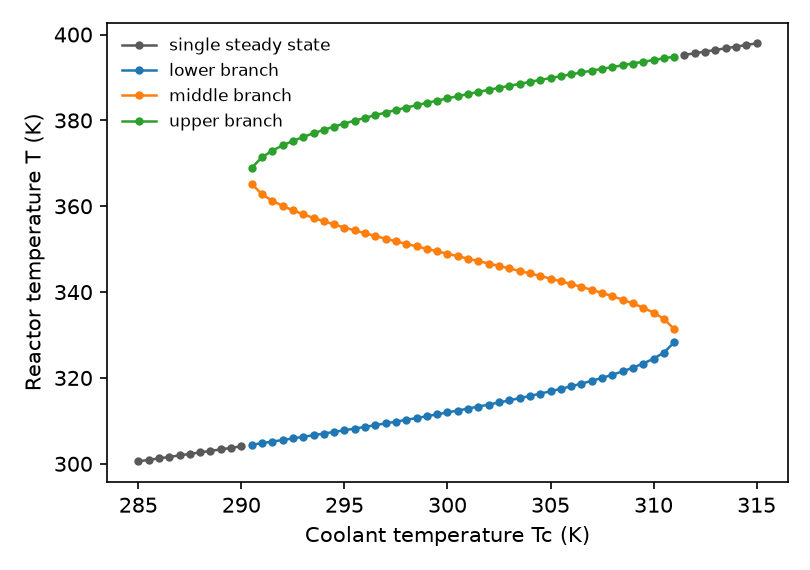
\includegraphics[width=\linewidth,height=5.5cm,keepaspectratio]{figures/cstr_steady_state_locus.png}
    \end{column}
    \begin{column}{0.31\textwidth}
      \begin{itemize}\setlength\itemsep{0.9em}
        \item At $T_c=300$ K, the notebook finds reactor temperatures near 312, 349, and 385 K.
        \item Three states appear from $T_c=290.5$ to 311 K on this grid.
        \item These are steady-state solutions, not stability results.
      \end{itemize}
    \end{column}
  \end{columns}
  \vfill
  \ndlogonote{\scriptsize Original notebook output; teaching parameters; 0.5 K sweep resolution}
\end{frame}
